\documentclass[11pt]{scrartcl}
\usepackage{tikz}
\usetikzlibrary{shapes.multipart, positioning}

\begin{document}

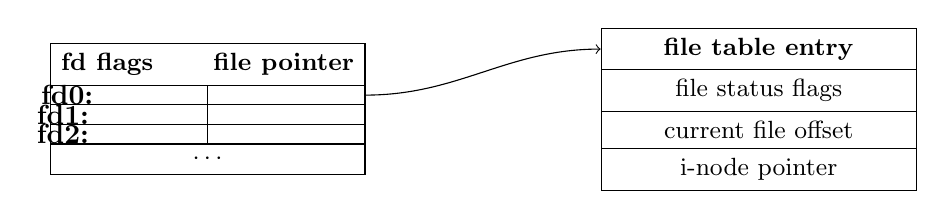
\begin{tikzpicture}
  \node[rectangle split, rectangle split parts=5, 
  draw, minimum width=4cm, font=\small,
  rectangle split part align={center}] (t1)
  { \textbf{fd flags} \hspace*{4ex} \textbf{file pointer}
    \nodepart{two}
    ~\hspace*{4ex}  
    \nodepart{three}
    ~ \hspace*{4ex}  
    \nodepart{four}
    ~ \hspace*{4ex}  
    \nodepart{five}
    $\cdots$};
  \draw (t1.text split) -- (t1.two split);
  \draw (t1.two split) -- (t1.three split);
  \draw (t1.three split) -- (t1.four split);
  \node[left=of t1.two] {\textbf{fd0:}};
  \node[left=of t1.three] {\textbf{fd1:}};
  \node[left=of t1.four] {\textbf{fd2:}};

  \begin{scope}[xshift=7cm]
    \node[rectangle split, rectangle split parts=4,
    draw, minimum width=4cm,font=\small,
    rectangle split part align={center}] (t2)
    {                \textbf{file table entry}
      \nodepart[label={fd1:}]{two} file status flags
      \nodepart{three} current file offset
      \nodepart{four} i-node pointer
    }; 
  \end{scope}
  \draw[->] (t1.two east) to [out=0, in=180](t2.text west);      
\end{tikzpicture}
\end{document}   

%%% Local Variables: 
%%% mode: latex
%%% TeX-master: t
%%% End: 
